% ============================================================
%  SCHOLA DOMESTICA — Magister Mathematica
%  Level 1 | Week 11 | Day 1
%  Topic: Addition Facts — +6 and +7, Sums to 10
% ============================================================
\documentclass[12pt, letterpaper]{article}

\usepackage[top=1in, bottom=1in, left=1in, right=1in]{geometry}
\usepackage[T1]{fontenc}
\usepackage[utf8]{inputenc}
\usepackage{lmodern}
\usepackage{microtype}
\usepackage{amsmath}
\usepackage{xcolor}
\usepackage{tikz}
\usepackage{array}
\usepackage{enumitem}
\usepackage{multicol}
\usepackage{mdframed}
\usepackage{fancyhdr}

\definecolor{scholared}{RGB}{160,30,30}
\definecolor{scholagold}{RGB}{180,140,40}
\definecolor{scholacream}{RGB}{253,248,235}
\definecolor{scholagreen}{RGB}{50,110,60}
\definecolor{scholablue}{RGB}{40,80,140}

\pagestyle{fancy}
\fancyhf{}
\renewcommand{\headrulewidth}{0.6pt}
\fancyhead[L]{\small\textcolor{scholared}{\textbf{Schola Domestica — Magister Mathematica}}}
\fancyhead[R]{\small\textcolor{scholared}{Level 1 · Week 11 · Day 1}}
\fancyfoot[C]{\small\textcolor{gray}{— \thepage\ —}}

\newcommand{\answerline}{\underline{\hspace{2.5cm}}}
\newcommand{\biganswerline}{\underline{\hspace{4cm}}}
\newcommand{\numbox}{\tikz{\draw[scholablue,thick](0,0)rectangle(1.2cm,0.85cm);}}

\newmdenv[
  backgroundcolor=scholacream,
  linecolor=scholared,
  linewidth=1.5pt,
  roundcorner=6pt,
  innertopmargin=8pt,
  innerbottommargin=8pt,
  innerleftmargin=10pt,
  innerrightmargin=10pt
]{lessonbox}

\newmdenv[
  backgroundcolor={rgb,255:red,235;green,245;blue,235},
  linecolor=scholagreen,
  linewidth=1.2pt,
  roundcorner=4pt,
  innertopmargin=6pt,
  innerbottommargin=6pt,
  innerleftmargin=8pt,
  innerrightmargin=8pt
]{enrichbox}

\begin{document}

\begin{center}
  {\LARGE\textbf{\textcolor{scholared}{Adding Six and Seven:}}}\\[4pt]
  {\Large\textcolor{scholagold}{\textit{Reaching Ten!}}}\\[6pt]
  {\small Name: \biganswerline \hspace{1cm} Date: \answerline}
\end{center}

\vspace{4pt}
\noindent\textcolor{scholared}{\rule{\linewidth}{1pt}}
\vspace{4pt}

% IMAGE PROMPT (Miyazaki watercolour style):
% Ten fireflies glow over a quiet night pond — six clustered on the left bank, four drifting right.
% Deep indigo sky, reflected gold lights in still water, white paper background, no text.

\begin{lessonbox}
\textbf{Strategy: Turn the fact around, then count on.}\\[4pt]
\begin{itemize}[leftmargin=1.5em, itemsep=3pt]
  \item $3 + 6$: turn it to $6 + 3$ (start at 6, count on 3) $= 9$
  \item $2 + 7$: turn it to $7 + 2$ (start at 7, count on 2) $= 9$
\end{itemize}
\medskip
\noindent Always start counting from the \emph{bigger} addend — it saves steps!
\end{lessonbox}

\bigskip

% Number line 0–10
\noindent
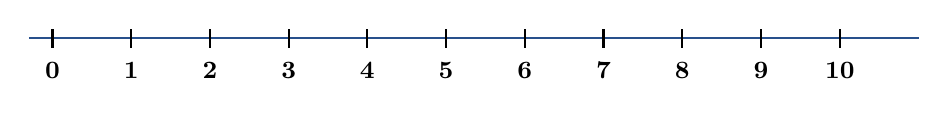
\begin{tikzpicture}
  \draw[thick, scholablue] (0,0) -- (11.3,0);
  \foreach \n in {0,...,10} {
    \draw[thick] (\n*1.0+0.3, -0.12) -- (\n*1.0+0.3, 0.12);
    \node[below] at (\n*1.0+0.3, -0.18) {\small\textbf{\n}};
  }
\end{tikzpicture}

\bigskip

% ===== PART I: +6 FACTS =====
\noindent\textcolor{scholared}{\large\textbf{Part I — Adding Six}} \hfill \textit{(Problems 1–5)}

\medskip
\noindent\textit{Use the number line or count on. Write the sum.}

\bigskip

\noindent
\begin{tabular}{@{}p{3.5cm} p{3.5cm} p{3.5cm} p{3.5cm}@{}}
\textbf{1.}\; $0 + 6 =$ \numbox &
\textbf{2.}\; $1 + 6 =$ \numbox &
\textbf{3.}\; $2 + 6 =$ \numbox &
\textbf{4.}\; $3 + 6 =$ \numbox
\end{tabular}

\medskip
\noindent\textbf{5.} $4 + 6 =$ \numbox \quad \textit{(what famous number does this make?)}

\bigskip\bigskip

% ===== PART II: +7 FACTS =====
\noindent\textcolor{scholared}{\large\textbf{Part II — Adding Seven}} \hfill \textit{(Problems 6–9)}

\bigskip

\noindent
\begin{tabular}{@{}p{3.5cm} p{3.5cm} p{3.5cm} p{3.5cm}@{}}
\textbf{6.}\; $0 + 7 =$ \numbox &
\textbf{7.}\; $1 + 7 =$ \numbox &
\textbf{8.}\; $2 + 7 =$ \numbox &
\textbf{9.}\; $3 + 7 =$ \numbox
\end{tabular}

\bigskip\bigskip

% ===== PART III: TURNAROUND PRACTICE =====
\noindent\textcolor{scholared}{\large\textbf{Part III — Turn It Around}} \hfill \textit{(Problems 10–13)}

\medskip
\noindent\textit{Write the turned-around fact. Both should have the same answer.}

\bigskip

\noindent
\begin{tabular}{@{}p{7.2cm} p{7.2cm}@{}}
\textbf{10.}\; $3 + 6 =$ \numbox \quad and \quad $6 + 3 =$ \numbox &
\textbf{11.}\; $2 + 7 =$ \numbox \quad and \quad $7 + 2 =$ \numbox \\[14pt]
\textbf{12.}\; $4 + 6 =$ \numbox \quad and \quad $6 + 4 =$ \numbox &
\textbf{13.}\; $1 + 7 =$ \numbox \quad and \quad $7 + 1 =$ \numbox
\end{tabular}

\bigskip\bigskip

% ===== PART IV: WORD PROBLEMS =====
\noindent\textcolor{scholared}{\large\textbf{Part IV — Story Problems}} \hfill \textit{(Problems 14–16)}

\medskip

\noindent\textbf{14.} A jar has \textbf{6} raisins. Mother adds \textbf{3} more. How many raisins?

\medskip\noindent\hspace{2em} $\numbox + \numbox = \numbox$ raisins

\bigskip

\noindent\textbf{15.} Seven butterflies sit on a flower. Two more land. How many butterflies?

\medskip\noindent\hspace{2em} $\numbox + \numbox = \numbox$ butterflies

\bigskip

\noindent\textbf{16.} Father has \textbf{4} nails and needs \textbf{10} in all. How many more does he need?

\medskip\noindent\hspace{2em} $4 +$ \numbox $= 10$\quad He needs \numbox\ more nails.

\bigskip

\begin{enrichbox}
\textbf{\textcolor{scholagreen}{Pairs That Make Ten}}\\[3pt]
These pairs always add to 10 — learn them like a song!\\[4pt]
$0+10=10$ \quad $1+9=10$ \quad $2+8=10$ \quad $3+7=10$ \quad $4+6=10$ \quad $5+5=10$\\[3pt]
\textit{We will finish all the ``ten pairs'' this week.}
\end{enrichbox}

\vspace{0.3cm}
\noindent\textcolor{gray}{\small\textit{Ray's Primary Arithmetic — counting on from the larger number.}}

\end{document}
